\section{Experimental Results}\label{sec:exp}
%
In this section, we present our experimental setup and the impact of the different optimizations and implementations described in the previous section.
\par\medskip
%
Figure \ref{fig:strongscaling_randomlin} shows the strong scaling behavior for the discussed algorithms.


\begin{figure}[ht]
	\centering
	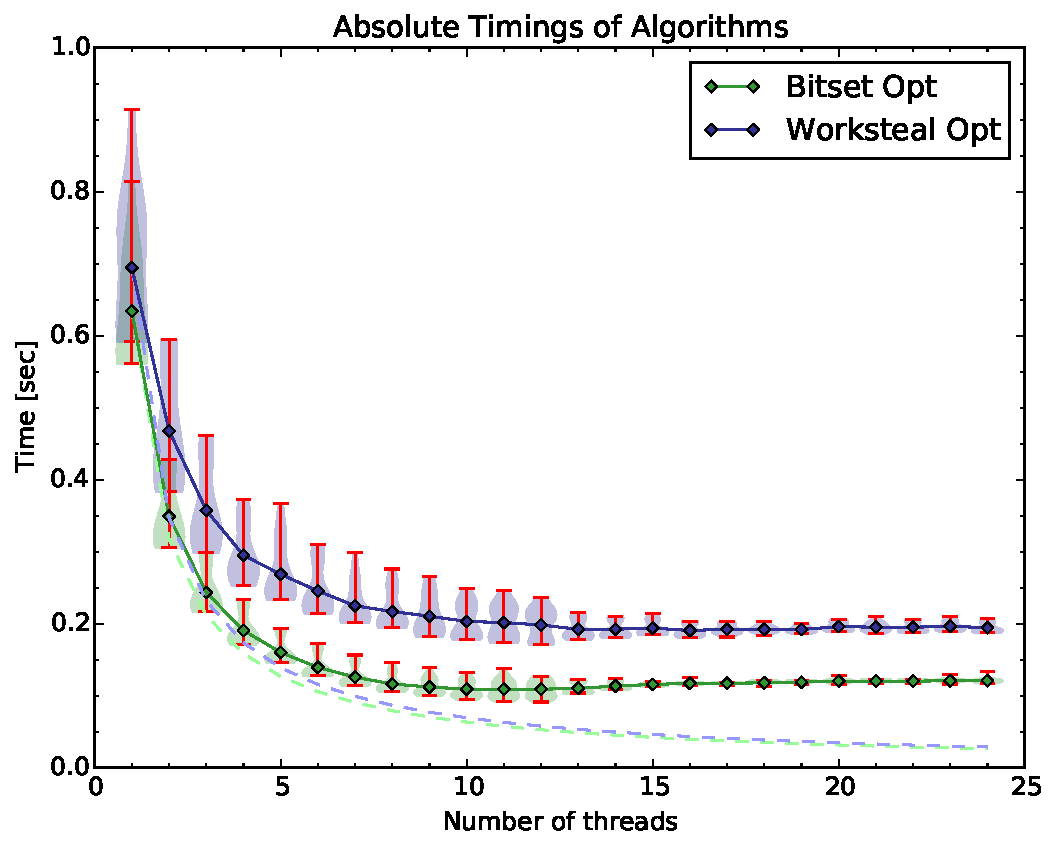
\includegraphics[width=\columnwidth]{plots/abstimings_comparison_gtSOFTWARE.pdf}
	\caption{<+caption text+>}
	\label{fig:<+label+>}
\end{figure}
\begin{figure}[ht]
	\centering
	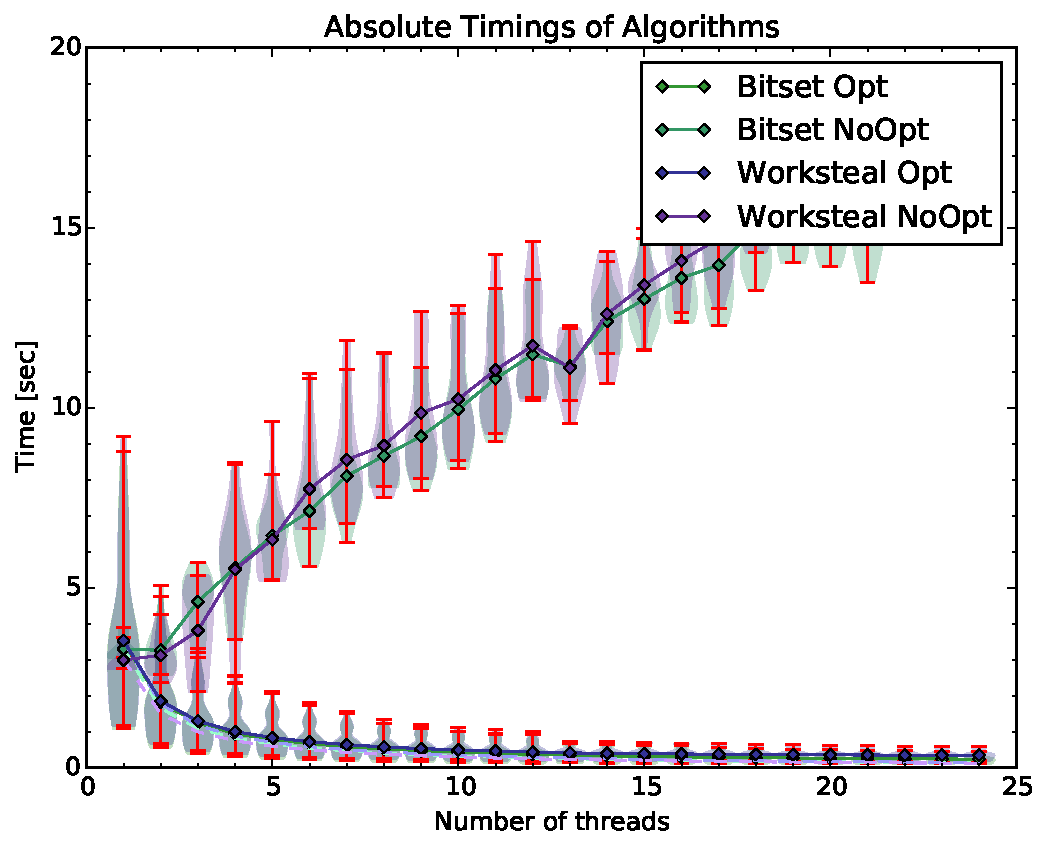
\includegraphics[width=\columnwidth]{plots/abstimings_comparison_gtRANDOMLIN.pdf}
	\caption{<+caption text+>}
	\label{fig:<+label+>}
\end{figure}
\begin{figure}[ht]
	\centering
	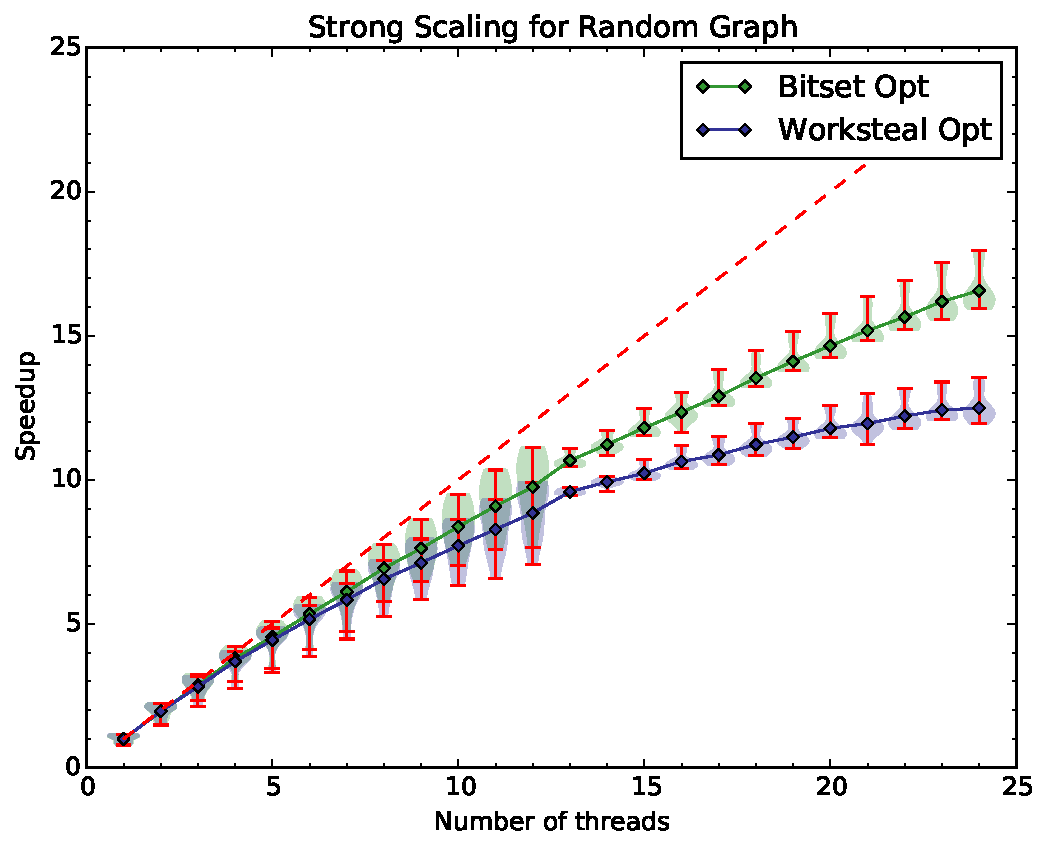
\includegraphics[width=\columnwidth]{plots/strongscaling_gtRANDOMLIN.pdf}
	\caption{<+caption text+>}
	\label{fig:strongscaling_gtrandom}
\end{figure}
\begin{figure}[ht]
	\centering
	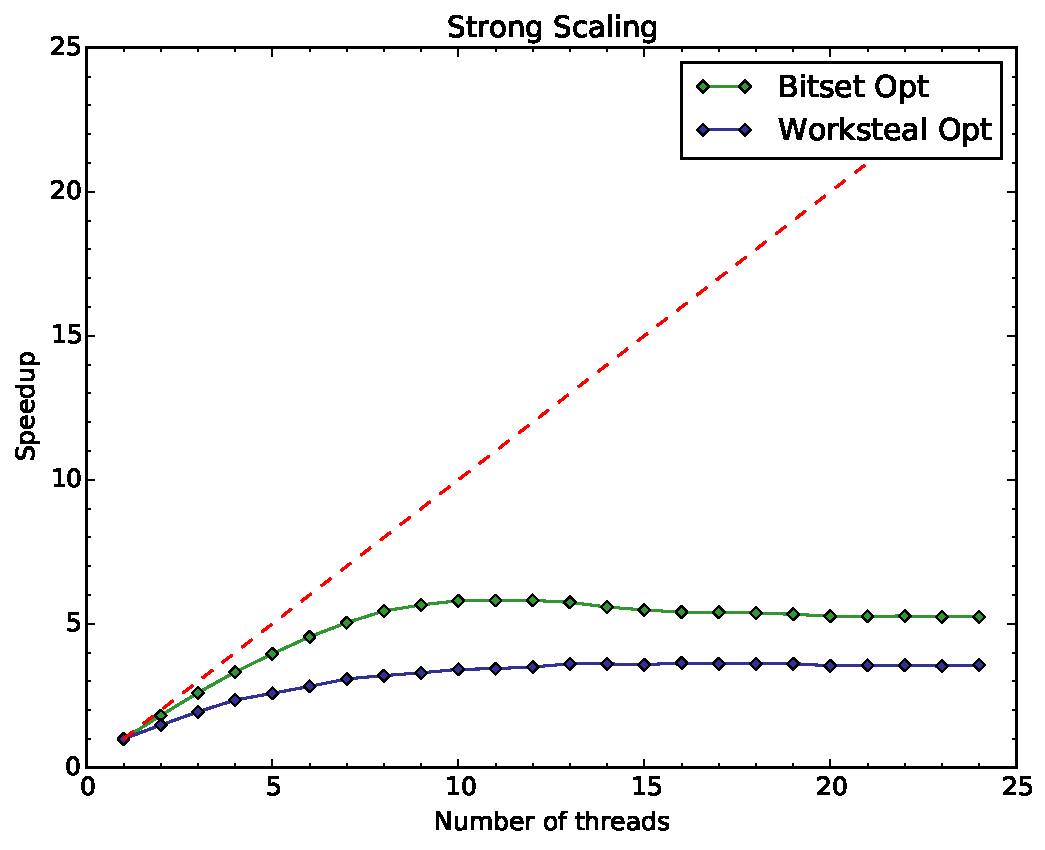
\includegraphics[width=\columnwidth]{plots/strongscaling_gtSOFTWARE.pdf}
	\caption{<+caption text+>}
	\label{fig:strongscaling_gtsoftware}
\end{figure}
\begin{figure}[ht]
	\centering
	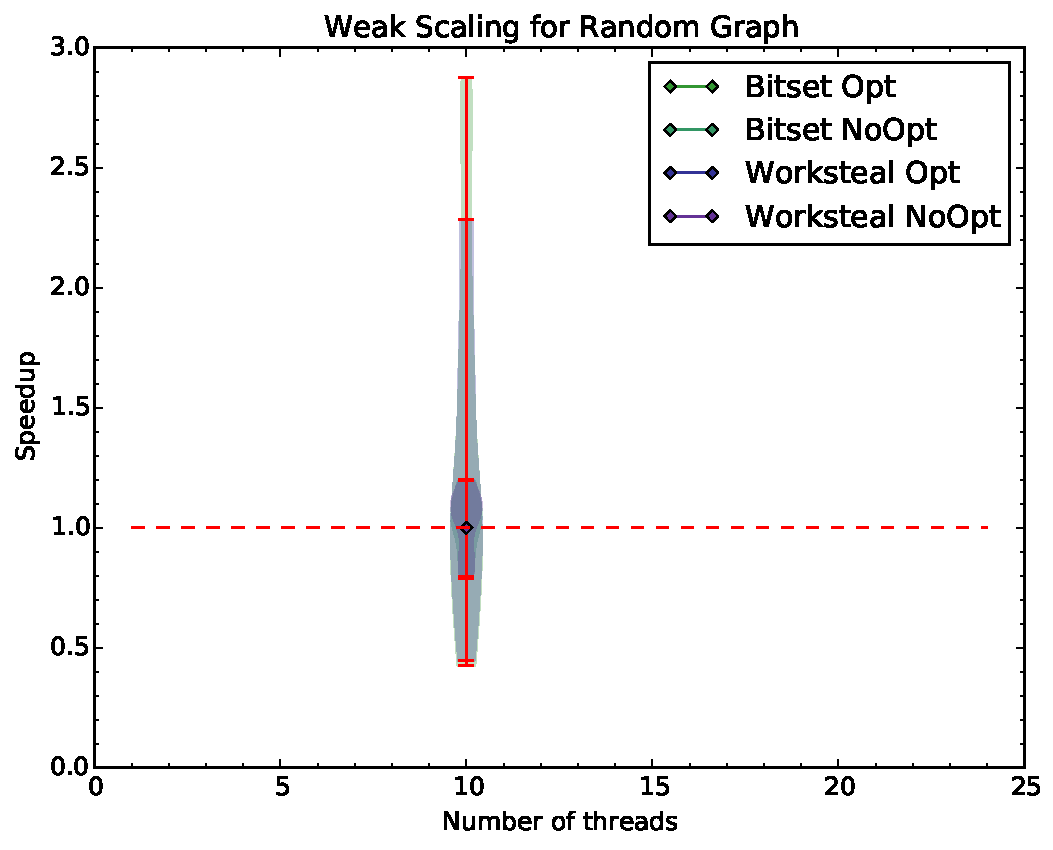
\includegraphics[width=\columnwidth]{plots/weakscaling_gtRANDOMLIN.pdf}
	\caption{<+caption text+>}
	\label{fig:<+label+>}
\end{figure}
\begin{figure}[ht]
	\centering
	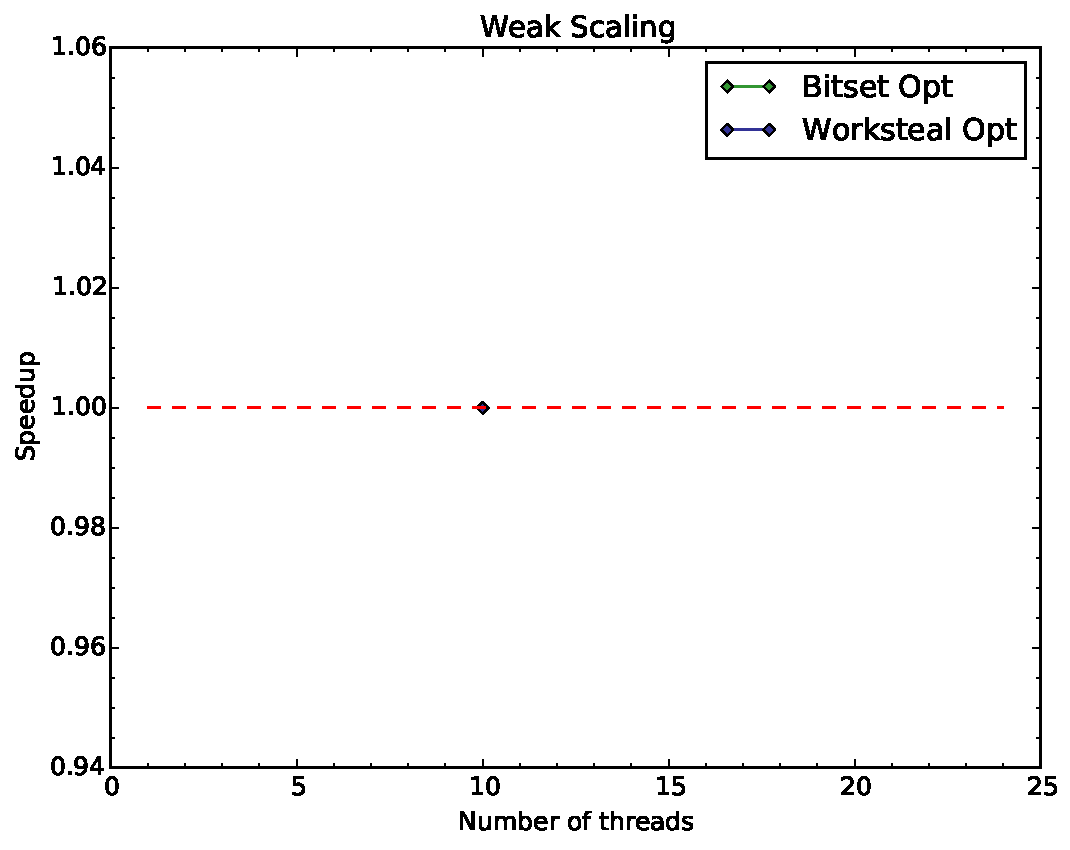
\includegraphics[width=\columnwidth]{plots/weakscaling_gtSOFTWARE.pdf}
	\caption{<+caption text+>}
	\label{fig:<+label+>}
\end{figure}
 \mypar{Hardware and compiler}
  \begin{table}[h]
    \centering
    \begin{tabular}{ll}
    \toprule
    Processor        & Intel Xeon E5-2697 (Ivy bridge) \\
    Max. clock rate  & 3.5 GHz (with TurboBoost)\\
    \# Sockets       & 2 \\
    Cores / socket   & 12 \\
    Threads / socket & 24 \\
    LLC / socket     & 30 MB \\
    \midrule
    Compiler and flags & GCC 4.8.2, -O3\\
    \bottomrule
    \end{tabular}
    \caption{Hardware and compiler used for benchmarks}
    \label{tab:hardware}
  \end{table}
 
 The following experiments were run on a 24-core system consisting of 2 Intel Xeon E5 processors (see table \ref{tab:hardware}).
 Hyperthreading was not used for the benchmarks.
 The implementations were written in \Cpp, using OpenMP and GCC atomic built-in functions. The graph was stored in an adjacency list.
\begin{invisible}

 \mypar{Benchmarks}
 For each item, mention graph type, number of nodes, node degree, optimizations from above
 \begin{itemize}
  \item Influence of barrier. Introduce multichain graph, Strong Scaling dynamic nobarrier opt2 MULTICHAIN100 vs bitset global opt1 MULTICHAIN100 Why Multichain100: Should be dominated by barrier%bitset_global is bitset without local solutions, because dynamic_nobarrier has no local solutions
  \item Influence of local solution. Strong Scaling bitset MULTICHAIN10000 vs bitset global MULTICHAIN10000 Why Multichain10000: Should be dominated by pushbacks to solution
  \item Influence of atomic counter check. Strong Scaling RANDOMLIN 100000 opt = true vs opt = false for worksteal and bitset
  \item Strong Scaling software graph \cite{musco2014generative}
  \item Strong Scaling random graph with different degrees
  \item Vertex Scaling plot random graph
 \end{itemize}

\mypar{Results}

Questions to each plot
\begin{itemize}
 \item What is the performance penalty of the barrier?
 \item How well performs the local solution compared to locking the 
 \item How does the atomic counter check scale compared to the locked version?
 \item How does the best version of our code scale on a real-world example?
 \item How does the best version of our code scale in a slightly artificial scenario?
\end{itemize}
\end{invisible}
